\documentclass[aps,pra,reprint,superscriptaddress,nofootinbib]{revtex4-2}
\usepackage{amsmath,amssymb,booktabs}
\usepackage{graphicx}
\usepackage{xcolor}
\usepackage[colorlinks=true,allcolors=blue]{hyperref}
\hypersetup{
  pdfauthor={Berkay Y{\"u}ksel Sayim},
  pdftitle={Emulating the frames of a mutual-information witness with time-bin light, and how precise the optics must be},
  pdfsubject={quant-ph; long-range nonstabilizerness; time-bin photonics; modular data},
  pdfkeywords={mutual-information witness, nonstabilizerness, SU(2) at level k, Weil representation, temporal Talbot effect, time bins}
}
\newcommand{\TODO}[1]{\textcolor{red}{[TODO: #1]}}
\newcommand{\Z}{\mathbb{Z}}

\begin{document}
\title{Emulating the frames of a mutual-information witness with time-bin light, and how precise the optics must be}
\author{Berkay Y{\"u}ksel Sayim}
\email{berksa@tutamail.com}
\affiliation{Independent Research, Germany}
\affiliation{\href{https://orcid.org/0009-0004-4993-7352}{ORCID:
0009-0004-4993-7352}}

\begin{abstract}
Mutual information between distant regions of a topologically ordered state can witness long-range nonstabilizerness; for anyon states it takes an operational form: the state is certified when the Shannon entropy of the anyon-type distribution is not an integer in some frame generated by the modular matrices $S$ and $T$.
For SU(2)$_k$ these frames are Clifford operations on a single qudit of dimension $2(k+2)$, a discrete Fourier transform and a quadratic phase, for which Talbot-type optics has been proposed, and whose Fourier stage has been used on time bins.
We show that the entropy of the time-bin distribution equals the label entropy plus one bit in every frame, so the witness is read from bin intensities.
In a pre-registered calculation for $k=2$ and $4$, a naive certification rule falsely certifies blind labels in more than half of the runs at $10^4$ photons per frame; it does so in 45 to 50\,\% of the runs even without phase noise, and phase noise of $0.05$\,rad adds $12.5$ to $23.2$ percentage points.
In the many-photon limit a protected rule keeps its margin for phase errors up to $0.14$\,rad ($k=2$) and over the whole tested range up to $0.40$\,rad ($k=4$, beyond the predicted range, so this prediction is refuted), and for uniform background counts up to $7\,\%$ and $3.5\,\%$.
The frame $S$, which separates blind from non-blind labels for $k=2$ and $4$, needs no phase stage; the phase thresholds apply to rules that also evaluate frames with a phase stage.
An independently written second implementation reaches the same pre-registered verdicts.
This is a proposal and a calculation, not an experiment: a single qudit can be emulated with classical light, so the scheme reproduces the frame structure of the witness and does not certify magic.
\end{abstract}
\maketitle

\begin{figure*}[t]
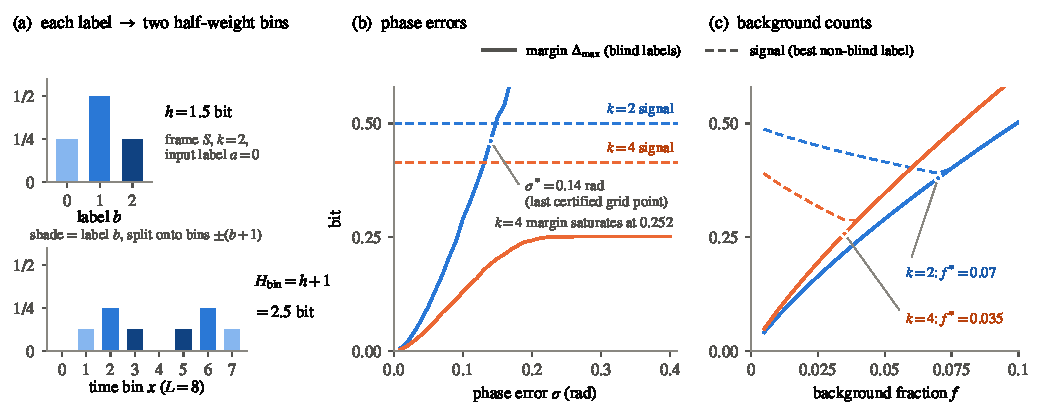
\includegraphics[width=\textwidth]{a_fig1_hero.pdf}
\caption{\label{fig:hero}(a) A label distribution on time bins, for $k=2$ and input label $a=0$ in the frame $S$ (direct calculation): the probability of each output label $b$ is split in half onto the bins $\pm(b+1)$ (same shade), the bins $0$ and $L/2$ stay empty, and the bin entropy is the label entropy plus one bit. (b) Protected rule under phase errors, many-photon limit: the margin $\Delta_{\max}$, the largest deviation a blind label can show (here the $99.865\,\%$ quantile under phase noise; solid), against the best noise-free distance of a non-blind label from the nearest integer (dashed, ``signal''), for $k=2$ (blue) and $k=4$ (orange). Among the seven frames used, phase errors change the intensities only in the frame $ST$; the frame $S$, which separates blind from non-blind labels for $k=2$ and $4$, needs no phase stage, so $\sigma^*$ applies to rules that also evaluate $ST$. For $k=2$ the signal stays above the margin up to $\sigma^*=0.14$\,rad (grid step $0.01$\,rad); for $k=4$ the margin saturates at $0.252$, below the signal $0.415$, up to the largest tested $\sigma=0.40$\,rad (so the censored value lies outside the predicted range; see text). The comparison uses the noise-free signal; it does not state that a single noisy measurement certifies. (c) The same comparison for a uniform background fraction $f$, with the background-shifted distance of a non-blind label as signal (dashed): $f^*=0.07$ ($k=2$) and $0.035$ ($k=4$), shown for $f\le0.1$. The dashed curves end where they meet the margin: just beyond, as long as the margin stays below $0.5$ bit, the largest distance comes from frames in which every label has integer entropy and equals the margin; it does not exceed the margin again up to $f=0.4$. Panels (b) and (c): data of the pre-registered run. A model calculation, not an experiment: the single-qudit emulation reproduces the frame structure of the witness, not a quantum resource.}
\end{figure*}

\section{Introduction}
Long-range nonstabilizerness (LRN) of topologically encoded states can be certified from the Shannon entropy of the state's coefficients in the minimally-entangled-state basis, evaluated after products of the modular matrices $S$ and $T$: if the entropy is not an integer in some frame, the state has LRN (Theorem~3 of Ref.~\cite{Korbany2026MI}).
For SU(2)$_k$ the modular matrices embed into the Clifford (Weil) representation of a single qudit of dimension $L=2(k+2)$: with $F_{xy}=e^{-2\pi ixy/L}/\sqrt L$ the discrete Fourier transform and $P=\mathrm{diag}(e^{i\pi x^2/L})$, one has $S=i\,U^\dagger FU$ and $T=e^{-i\pi/L}\,U^\dagger PU$, where $U$ maps label $m-1$ ($m=1,\dots,k+1$) to $u_m=(\delta_m-\delta_{-m})/\sqrt2$. Here $N=k+2$, $S_{ab}=\sqrt{2/N}\,\sin(\pi(a+1)(b+1)/N)$ and $T=\mathrm{diag}(\theta_a)$ with $\theta_a=e^{2\pi i\,a(a+2)/(4N)}$ (without the central-charge phase). Both identities follow in a few lines: $\langle u_m|F|u_{m'}\rangle=-(2i/\sqrt L)\sin(\pi mm'/N)$, and $2/\sqrt L=\sqrt{2/N}$, so $U^\dagger FU=-iS$; and $\theta_{m-1}=e^{2\pi i(m^2-1)/(4N)}=e^{-i\pi/L}\,e^{i\pi m^2/L}$. $F$ and $P$ commute with the parity $x\to-x$ and therefore preserve the odd subspace (dimension $k+1$), which is the image of $U$. For the general theory of Weil representations and of modular representations inside them see Refs.~\cite{EholzerSkoruppa1995,Cheng2024}; the computation above does not rely on it. We checked both identities numerically for $k=2$ and $4$ and, in the pre-registered test below, for $k\in\{5,7,8,9,11,12\}$ (largest deviation $7.4\times10^{-15}$).
In optics, $P$ is a quadratic phase and $F$ a Fourier transform over time or frequency bins.
Talbot-type optics has been proposed for such operations: in space, where free propagation together with a diagonal phase gate gives a complete set of single-qudit gates \cite{Farias2015}, and for Clifford gates on time--frequency GKP qubits \cite{Pousset2026}. On time bins, a temporal Talbot stage has been used in experiments as a Fourier detection in dimension 4 \cite{Widomski2024,Ogrodnik2025}.
Frequency-bin Fourier gates have been simulated up to dimension 10 and demonstrated for dimension 3 \cite{Lu2022}, and quadratic phases are available from dispersion and electro-optic time lenses \cite{LipkaParniak2023}.
Photonic simulators have also emulated anyon physics: a classical photonic simulator encoding a single qutrit reproduced the fusion and braiding of $D(S_3)$ anyons \cite{Goel2024}, and Clifford operator Berry phases corresponding to the braiding of parafermions were emulated with photonic states \cite{Liu2021}.
Using these operations as gates is not new; here we use them to emulate the frames of the witness.
\emph{We ask:} can the frames of the witness be emulated on a time-bin qudit, and how precise must the optical elements be so that integer and non-integer values remain distinguishable?
\emph{What we do not claim:} an experiment; a certificate of magic in light (for a single qudit, classical light suffices, so the emulation reproduces the frame structure, not a quantum resource).

\section{Mapping}
\paragraph*{Bins and labels.}
Label $a$ is encoded as $Ue_a=(\delta_m-\delta_{-m})/\sqrt2$ on $L$ time bins, $m=a+1$.
Since $F$ and $P$ map odd functions to odd functions and act on them as $S$ and $T$ up to phases, a word in $F$ and $P$ maps $Ue_a$ to $U(Me_a)$ up to a phase, where $M$ is the same word in $S$ and $T$.
Each label amplitude $c_b$ of $Me_a$ is split with equal weight $|c_b|^2/2$ onto the two bins $\pm(b+1)$, so every probability of the label distribution is halved and doubled in number:
\begin{equation}
H_{\rm bin}=h_a(M)+1
\end{equation}
exactly, for every frame (illustrated in Fig.~\ref{fig:hero}a). The witness is therefore read from the bin intensities with a constant offset of one bit.

\emph{Pre-registered test (A1).} Before computing them we fixed the test set $k\in\{5,7,8,9,11,12\}$, all 127 words of length $\le6$, and the criterion that both $|H_{\rm bin}-h_a-1|$ and the matrix identities above deviate by less than $10^{-12}$.
The largest deviations are $3.0\times10^{-14}$ (entropy) and $7.4\times10^{-15}$ (matrices); A1 is confirmed.
A negative control with the even embedding $(\delta_m+\delta_{-m})/\sqrt2$ breaks the matrix identities (deviation $0.71$ for $k=2$, $0.58$ for $k=4$), but at $k=2$ it leaves the entropy identity intact for all words up to length 4 ($3.6\times10^{-15}$), while at $k=4$ it breaks it ($0.25$): entropies alone do not always fix the embedding, which is why the matrix form is part of the test.
\paragraph*{Doubled theory.}
By the doubled theory of a modular category $\mathcal C$ we mean its center $Z(\mathcal C)$; for modular $\mathcal C$ one has $Z(\mathcal C)\simeq\mathcal C\boxtimes\tilde{\mathcal C}$, with $\tilde{\mathcal C}$ the category with reversed braiding \cite{Mueger2003}; hence $S_D=S\otimes\bar S$, $T_D=T\otimes\bar T$, and every frame of the doubled theory is $M\otimes\bar M$.
For a product MES $(i,\bar j)$ the flux distribution in such a frame is the product of $|Me_i|^2$ and $|\bar Me_j|^2=|Me_j|^2$, and Shannon entropy is additive on products: the witness value is $h_i(M)+h_j(M)$, so two single-qudit runs in the same frame suffice.

\newif\ifblindtable
\blindtabletrue
\ifblindtable
\paragraph*{Blind labels for $k=2$ and $k=4$.}
We list the labels and product pairs whose witness value is an integer in every frame (Table~\ref{tab:blind}); this analysis is not part of the pre-registration.
\emph{Method:} we generate the full frame group $\langle S,T\rangle$ up to a global phase (384 elements for $k=2$, 2304 for $k=4$), evaluate the entropies in floating point, and call a value integer if it lies within $10^{-9}$ of an integer; for every non-blind label or pair, the largest distance from an integer over the frame group is at least $0.20$ ($k=2$) and $0.169$ ($k=4$), far above the tolerance (for a label $i$ this follows from the pair of $i$ with a blind label).
For $k=2$ the seven frames of length $\le2$ used below suffice for single labels but not for pairs: the pairs $(0,\bar0)$, $(0,\bar2)$, $(2,\bar0)$ and $(2,\bar2)$ have integer values in all seven and first become non-integer in the frame $STTS$ (distance $0.20$).
We make no statement beyond $k=2$ and $k=4$.
\begin{table}[b]
\caption{\label{tab:blind}Labels $a=0,\dots,k$ of SU(2)$_k$ and product pairs $(i,\bar j)$ of the doubled theory whose witness value is an integer in every frame.}
\begin{ruledtabular}
\begin{tabular}{ccc}
$k$ & blind labels & blind pairs $(i,\bar j)$\\
\hline
2 & $1$ & $(1,\bar1)$\\
4 & $1,\ 3$ & $(1,\bar1),\ (1,\bar3),\ (3,\bar1),\ (3,\bar3)$\\
\end{tabular}
\end{ruledtabular}
\end{table}
\fi

\section{Error budget}\label{sec:budget}
\paragraph*{Model and rules.}
Each application of $P$ carries independent Gaussian phase errors $\phi_x\sim\mathcal N(0,\sigma^2)$ on every bin, static during the acquisition of one frame and drawn anew for every frame and repetition.
Background counts are modeled as a fraction $f$ of all detected counts spread uniformly over the $L$ bins.
The label entropy is estimated as the plug-in bin entropy with the Miller--Madow correction, minus one bit, with $\hat\sigma$ from the delta method.
A \emph{naive} rule certifies a state if $|\hat H-\mathrm{nint}(\hat H)|-3\hat\sigma>0$ in any of the seven frames $\mathrm{id},S,T,SS,ST,TS,TT$; a \emph{protected} rule requires $|\hat H-\mathrm{nint}(\hat H)|>\Delta_{\max}+3\hat\sigma$, where $\Delta_{\max}$ is the largest deviation a blind label can show: the $99.865\,\%$ quantile under phase noise ($10^5$ draws), or the deterministic shift under background counts.
The settings, ranges and decision criteria of the tests (a)--(c) below were fixed in a pre-registration before the computation. It followed exploratory runs of the same code on other cases, and its predicted ranges are wide. The analysis of where phase errors act, the second-route comparison and the paragraphs marked as addendum were added afterwards.

\paragraph*{Where phase errors act.}
Phase errors change the bin intensities only if a phase stage is followed by a Fourier stage; among the seven frames this happens only in $ST$.
There they enter only through the difference $\Delta=\phi_m-\phi_{-m}\sim\mathcal N(0,2\sigma^2)$ of the two bins that carry a label.
In label space $S$, $ST$ and $TS$ give identical entropies (Table~\ref{tab:words}), so the non-blind labels for $k=2$ and $4$ are already detected in the frame $S$, which contains no phase stage.

\paragraph*{Results (A2).}
\emph{(a) Naive rule.} At $\sigma=0.05$\,rad and $N_{\rm ph}=10^4$ photons per frame, blind labels are falsely certified in $73.4\,\%$ of 1000 repetitions for $k=2$ (label 1) and in $57.9\,\%$ and $60.4\,\%$ for $k=4$ (labels 1 and 3); the prediction of at least $50\,\%$ for every blind label is confirmed.
Without phase noise the same rule still fires in $50.2\,\%$, $45.4\,\%$ and $45.9\,\%$ of the runs, so most of the failure comes from the estimator; phase noise adds $23.2$, $12.5$ and $14.5$ percentage points. A plausible mechanism, not tested separately here: the bin distribution of a blind label is uniform on its support, where the first-order variance estimate is close to zero while the bias does not vanish.
Since this control reaches $50\,\%$ at $k=2$ in the pre-registered run, the pre-registered rule does not attribute the false certificates at $k=2$ to phase noise. The control lies at this threshold: the second implementation (below) gives $46.2\,\%$, and (addendum, not part of the pre-registration) a run with 40\,000 repetitions gives $47.5\,\%\pm0.25\,\%$.

\emph{(b) Protected rule, phase errors.} With many photons, the best noise-free distance of a non-blind label ($0.5$ for $k=2$, labels 0 and 2 in $S$; $0.415$ for $k=4$, label 2) exceeds $\Delta_{\max}(\sigma)$ up to $\sigma^*=0.14$\,rad for $k=2$, inside the predicted range $[0.02,0.30]$\,rad.
For $k=4$, $\Delta_{\max}$ saturates at $0.252$, below $0.415$, so the condition holds on the whole grid up to $0.40$\,rad; by the pre-registered rule this censored value lies outside the predicted range, and the prediction is refuted for $k=4$ in the favorable direction; A2(b) is therefore partially confirmed (Fig.~\ref{fig:hero}b).
The comparison uses the noise-free distance: it states that the margin stays below the clean signal, not that a single noisy measurement certifies.

\emph{(c) Protected rule, background counts.} In the many-photon limit, comparing the background-shifted distance of a non-blind label with the deterministic margin, the rule keeps a non-blind label certifiable up to $f^*=0.07$ for $k=2$ and $f^*=0.035$ for $k=4$, both inside the predicted range $[0.01,0.30]$; the prediction is confirmed (Fig.~\ref{fig:hero}c).

\emph{Second route.} An independently written second implementation, deposited with this record, repeats the calculation and computes $\Delta_{\max}(\sigma)$ without sampling error from the density of $|\Delta|$; the values it reports are transcribed in the comparison script of this record. Its verdicts on (a)--(c) are the same as above; one of the comparison bounds set in advance is exceeded, at $k=2$, $\sigma=0.02$, where $\Delta_{\max}$ is small and the two values ($0.0208$ and $0.0213$) differ by $2.4\,\%$ against a bound of $2\,\%$, and its background margins agree with ours to the four digits it reports. (Addendum, computed with the code of this record: on the whole $\sigma$ grid the 80 Monte Carlo values of $\Delta_{\max}$ lie within $3.2\,\%$ of the sampling-free quantile, largest at $k=4$, $\sigma=0.07$\,rad; the mean signed deviation is $+0.1\,\%$, the spread $1.0\,\%$ for $k=2$ and $0.8\,\%$ for $k=4$.)

\section{Components}
Table~\ref{tab:words} lists the seven frames with their optical stages for $L=8$ bins ($k=2$) and $L=12$ bins ($k=4$).
\begin{table}[t]
\caption{\label{tab:words}Frames of length $\le2$ ($XY$: first $Y$, then $X$), number of Fourier ($F$) and phase ($P$) stages, whether a phase stage precedes a Fourier stage (only then phase errors change the intensities), and the largest distance of a label entropy from the nearest integer.}
\begin{ruledtabular}
\begin{tabular}{lccccc}
frame & $F$ & $P$ & $P$ before $F$ & $k=2$ & $k=4$\\
\hline
id & 0 & 0 & no & 0 & 0\\
$S$ & 1 & 0 & no & 0.500 & 0.415\\
$T$ & 0 & 1 & no & 0 & 0\\
$SS$ & 2 & 0 & no & 0 & 0\\
$ST$ & 1 & 1 & yes & 0.500 & 0.415\\
$TS$ & 1 & 1 & no & 0.500 & 0.415\\
$TT$ & 0 & 2 & no & 0 & 0\\
\end{tabular}
\end{ruledtabular}
\end{table}
For orientation we list reported component values, as citations only.
A temporal Talbot detection of time-bin superpositions in dimension 4 used a dispersion module with a group-delay dispersion of $12\,900$\,ps$^2$ and an insertion loss of $2.67$\,dB, detectors with an efficiency of $84\,\%$ according to the manufacturer, and a combined timing jitter of $11$\,ps rms \cite{Ogrodnik2025}.
A frequency-bin Fourier gate built from a three-component quantum frequency processor reaches a simulated gate fidelity above $0.9997$ with success probability above $0.965$ up to dimension 10, and was demonstrated for dimension 3 \cite{Lu2022}.
Dark-count probabilities of $2.8$ to $3.4\times10^{-7}$ enter the key-rate simulations of Ref.~\cite{Ogrodnik2025} as parameters; we did not find a number for the phase stability of a phase stage in the works read for this paper. The Talbot detection there is far from ideal: the reported error rates in the Fourier basis are about $22$ to $25\,\%$ in dimension 2 and about $36\,\%$ in dimension 4 \cite{Ogrodnik2025}, whereas our model assumes an ideal Fourier stage.
The dimensions needed here, $L=8$ for $k=2$ and $L=12$ for $k=4$, exceed those demonstrated for these stages in the works cited here (dimension 4 for temporal Talbot detection, dimension 3 for frequency-bin Fourier gates); the thresholds of Sec.~\ref{sec:budget} state how precise such stages would have to be, not that they exist.

\section{Discussion and limitations}
The emulation reproduces the frame structure of the witness, not a quantum resource: for a single qudit the bin probabilities, i.e.\ the mean bin intensities, of classical light are the same, so nothing here certifies magic in light; only the counting statistics differ, and the error budget above assumes single-photon counting.
For the doubled theory two single-qudit runs in the same frame suffice for product states, by the additivity above.
For single labels at $k=2$ and $4$ the frame $S$ alone separates blind from non-blind labels and needs no phase stage; the phase budget becomes relevant for states that require longer words with a phase stage before a Fourier stage.
Not modeled: errors of the Fourier stage itself, a systematic error of the quadratic coefficient (a mis-set dispersion or time lens), phase errors correlated between bins, detector timing jitter, and loss that depends on the bin; the background model is uniform.
The thresholds hold within this model: (a) at $10^4$ photons per frame, (b) and (c) in the many-photon limit, against the noise-free and the background-shifted distance, respectively.

\section*{Data and code availability}
The scripts and result files are deposited with this record (DOI \href{https://doi.org/10.5281/zenodo.23148214}{10.5281/zenodo.23148214}).
The pre-registration was locked before the computation; its SHA-256 hash (of the file with LF line endings) is \texttt{4a11d668456e974f99f71ab73cf2baf1}\allowbreak\texttt{6ae3a535ccdeba406bd878c374f0ffc9}. The pre-registration file itself is not part of this record.
Paper, figures, and data are released under the Creative Commons Attribution 4.0 International (CC~BY~4.0) license; the deposited source code is released under the Apache License 2.0 (see \texttt{LICENSE}).

\section*{Use of AI tools}
In the research, processing, and writing of this paper and its results I worked together with generative AI tools, in practice a system of multiple coordinated AI instances that I set up and orchestrate (large language models, mainly Claude, by Anthropic, inside Claude Code). At their current context sizes I found it far more effective to work with several specialized instances, each with its own role and its own harness of rules and parameters that I designed and refined through feedback, than to load a single instance with all of the material; for my workflow that would have been inefficient, though this depends on the individual implementation. I lead this collaboration: I choose the research directions, set the goals, and make the final decisions in open exchange with the AI, learning actively as the work proceeds. The AI carries out the drafting, including the mathematical and technical parts, the numerical computation, and the literature search, under my direction. The AI works autonomously only task by task, within the structure I develop through feedback: it completes a task, and at open questions that need me it stops until the point is settled before the next step. Along the way I witness and take many of the decisions that shape the path, and it is common for me to spot things that need improvement. The work spans many separate runs, and a single simulation or build task alone can take up to an hour, so it could not happen all together in one autonomous run; and had I let the AI do all of it together alone, even if it is possible, it would no longer be my work but the AI's.

I run multiple verifications at the different stages of the work and one before release, and all references are checked against the original sources. In the end what matters are human eyes, a principle that is itself written into the parameters of my system: I reach out to experts after publishing for review and feedback, so I learn what is solid and what must be corrected or falsified. My scripts for reproduction and review are released with this record. These tools are not authors; I am the author, and I take full responsibility for all scientific content and decisions leading to these results and their publication.

\section*{Acknowledgments}
This research received no specific grant from any funding agency in the public,
commercial, or not-for-profit sectors. The author declares no competing
interests.

\bibliography{talbot_refs}
\end{document}
